\documentclass[a4paper,10pt,twocolumn]{article}
	\usepackage{amsmath}
	\usepackage{graphicx}
	\usepackage{newtxtext,newtxmath}
	\usepackage{lipsum}
	\usepackage{tabularx}
	\usepackage{booktabs}
	\usepackage{algorithm}
	\usepackage{algorithmic}
	\usepackage{float}
	\usepackage{geometry}
	\usepackage{titling}
	\usepackage{makeidx}
	\usepackage{url}
	\usepackage{amsmath}
	\usepackage{nccmath} 
	\usepackage[title,titletoc]{appendix}
	\setlength{\parindent}{0pt}
	\geometry{
	a4paper,
	total={170mm,257mm},
	left=20mm,
	top=20mm,
	}
	\frenchspacing
	\renewcommand{\appendixname}{Appendix }
	\pretitle{%
	\begin{center}
	\LARGE
	
\includegraphics[width=40mm]{logo-min}\\[\bigskipamount]
	Aidos Kuneen \\ 
	\Large
	}
	\posttitle{
		\normalsize
		\end{center}}
	
	
	
	\title{--- A Blockless and Anonymous Cryptocurrency for the Post-Quantum Era ---}
	
	\author{
		Aidos Developer \and Aidos Foundation
	}
	\date{April, 2019 \\ Version 0.05 (DRAFT)}
	
	\begin{document}
	
	\twocolumn[
		\maketitle
	
	\begin{abstract}
			In this white paper we introduce a new cryptocurrency, \emph{Aidos Kuneen}. Aidos Kuneen has been developed to deliver 
			a fast, anonymous, blockless, decentralized and scalable solution for post-quantum era transfers with zero fees. 
	
	\vspace{2.5mm}
			
			Aidos Kuneen employs a mechanism known as \emph{iMesh}, within iMesh all transactions are directly referenced by
			one another in order to form a \emph{Directed Acyclic Graph (DAG)} structure.
	
	\vspace{2.5mm}
			
			The inclusion of `AKConsensus' allows full-nodes to determine which transactions are legitimate within the DAG structure 
			and to reject those that are not. AKConsensus provides fast payment by concurrent confirmation and resilience against any attackers who may happen to gain 
			control of up to 33\% of the validators.
	
	\vspace{2.5mm}
			
			To ensure continued security in the post-quantum era, Aidos Kuneen utilises the lattice-based signature `BLISS'. BLISS
			provides for both relatively small signature and public key size which in turn reduces network load.
	
	\vspace{2.5mm}
		
			In order to provide anonymity within the network, Aidos Kuneen employs \emph{AKShuffle}. AKShuffle 	
			incorporates stealth address inspired from CryptoNote and coin mixing, this allows for truly anonymous transfers 
			throughout the entire network.
	
	\vspace{2.5mm}
			
			To allow Aidos Kuneen to service the expected future growth of the `IoT' sector we introduce  
			`ticket mining' for a co-operative Proof of Work mechanism. This  allows a number of ticket miners within the network to 
			co-operatively perform the necessary Proof of Work in order to confirm transactions on the network, thus reducing 
			the physical processing requirements of any one sender when sending.
			
			\end{abstract}
	
			\vspace{1.5cm}
	
	\footnotesize
	Copyright \copyright2017--2019 by Aidos Developer and Aidos Foundation.
	
	\vspace{2mm}
		
	IN NO EVENT SHALL THE AUTHORS OR COPYRIGHT HOLDERS BE HELD LIABLE FOR ANY CLAIM, DAMAGES OR OTHER
	LIABILITY, WHETHER IN AN ACTION OF CONTRACT, TORT OR OTHERWISE, ARISING FROM,
	OUT OF, OR IN CONNECTION WITH THIS DOCUMENT, OR THE USE OF OR OTHER DEALINGS WITH
	THIS DOCUMENT\@.\\
	
	This work is licensed under a Creative Commons Attribution 4.0 International License. \\
	\url{http://creativecommons.org/licenses/by/4.0/} \\
	
\includegraphics{cc}
	]
	
	\normalsize
	\twocolumn[
	\tableofcontents
	\listoffigures
	]
	
	\clearpage
	
	\section{Introduction}
	Bitcoin, the once obscure cryptocurrency introduced by Satoshi Nakamoto~\cite{btc} in 2008, has now begun to draw much wider attention 
	from both the general public and governments alike. Within the Bitcoin network, transactions are written into `blocks', these blocks 
	are then cryptographically validated by powerful computers known as `miners' using a Proof of Work (PoW) system. Once a block has been 
	validated it is then appended to the end of a continually growing chain of blocks aptly named `the block-chain'. Miners are 
	subsequently rewarded for successfully validating a block by means of the transaction fees paid by senders who transact on the Bitcoin 
	network.\\
	
	Currently, blocks are added to the blockchain at a rate of approximately one every 10 minutes. The transactions contained within the
	blocks consist of both input and output addresses, with the inputs themselves being the outputs of previous transactions --- this 
	provides an auditable history of all past Bitcoin transactions within the network. In order to prove ownership, transactions are signed 
	by the address owner with an Elliptic Curve Digital Signature Algorithm (ECDSA).\\
	
	However, in recent years a number of problems have been identified with the Bitcoin implementation, including:
	\vspace{-0.5\baselineskip}
	\begin{itemize}
		\setlength\itemsep{0em}
		\item\textbf{Limited Scalability}\mbox{}\\ 
		Within the core Bitcoin code, the maximum block size is restricted and blocks are unable to store transactions once this limit 
		is exceeded. This in turn leads to a scalability problem when many transactions are broadcast simultaneously with many of them 
		being unable to be included in the current block.
		\item\textbf{High Transaction Fees}\mbox{}\\ 
		Senders are required to pay a transaction fee in order to incentivise the miners to include their transaction in a block.
		If Bitcoin usage continues to grow and the price of Bitcoin increases, the relative value of the fee will also increase.
		It no longer makes sense to send small transactions via the Bitcoin network
		as the fee could easily exceed the value of the Bitcoin being transacted. This forces senders to use complicated schemes to send small value transactions (e.g. 
		micropayment channels).
		\item\textbf{Poor Resistance Against Quantum Computers}\\ 
		As of 2019, the development of quantum computers is still in its infancy. However, experiments have already been carried out in 
		which quantum computational operations were executed on a small number of quantum bits. Furthermore, Google has reported its 
		intent to commercialize quantum technologies within the next five years~\cite{google}. At the same time, according to Shor's 
		algorithm~\cite{shor}, all algorithms based on the discrete logarithm problem (including ECDSA as used in 
		Bitcoin), can be easily solved with a sufficiently powerful quantum computer. 
		\item\textbf{Limited Anonymity}\mbox{}\\ 
		The auditable nature of Bitcoin means that in order to spend Bitcoin, the spending transaction must refer back to the founding
		transactions that came before it, these founding transactions are open to the public. As such, anyone is free to track the flow
		of BTC from address to address.
	\end{itemize}
	
	In order to address these issues, we introduce a new cryptocurrency, \emph{Aidos Kuneen}.
	The Aidos Kuneen network, known as \emph{iMesh}, is based on \emph{Directed Acyclic Graph (DAG)} technology.
	In iMesh, transactions are directly referred to by other transactions and as such there are no blocks, and by extension, no block-chain.
	iMesh allows doing confirmations concurrently, so we are able to achieve the benefits of scalability.
	
	\vspace{2.5mm}
	
	Adios Kuneen has been specifically designed to provide:
	\vspace{-0.5\baselineskip}
	\begin{itemize}
		\setlength\itemsep{0em}
		\item\textbf{Increased Scalability}\mbox{}\\ 
	In iMesh, one performs relatively simple PoW computations to confirm the transaction. After the transaction is broadcast to the network,
	the transaction is stored into iMesh immediately. Hence, there is no need to wait for one's own transaction to be stored. Additionally 
	there is no limitation to the size or number of transactions that can be stored at a time. 
	\item\textbf{Zero Fees}\mbox{}\\ 
	As one is no longer required to pay any transaction fees (owing to the fact that there are no miners), one is free to 
	transact with any amount, no matter how small without requiring any special knowledge or techniques.
	
	\item\textbf{Post-Quantum Resistance}\mbox{}\\ 
	In Aidos Kuneen we have specifically chosen a lattice-based signature which provides strong post-quantum security. There have been a 
	number of different signature architectures developed to provide resistance to future quantum based computer hardware, including 
	Hash-based, Multivariate, Code-based methods. However, the majority of these are not practical for our purposes due to their large key and 
	signature sizes.   
	
	
	\begin{figure}[ht]
		\begin{center}
		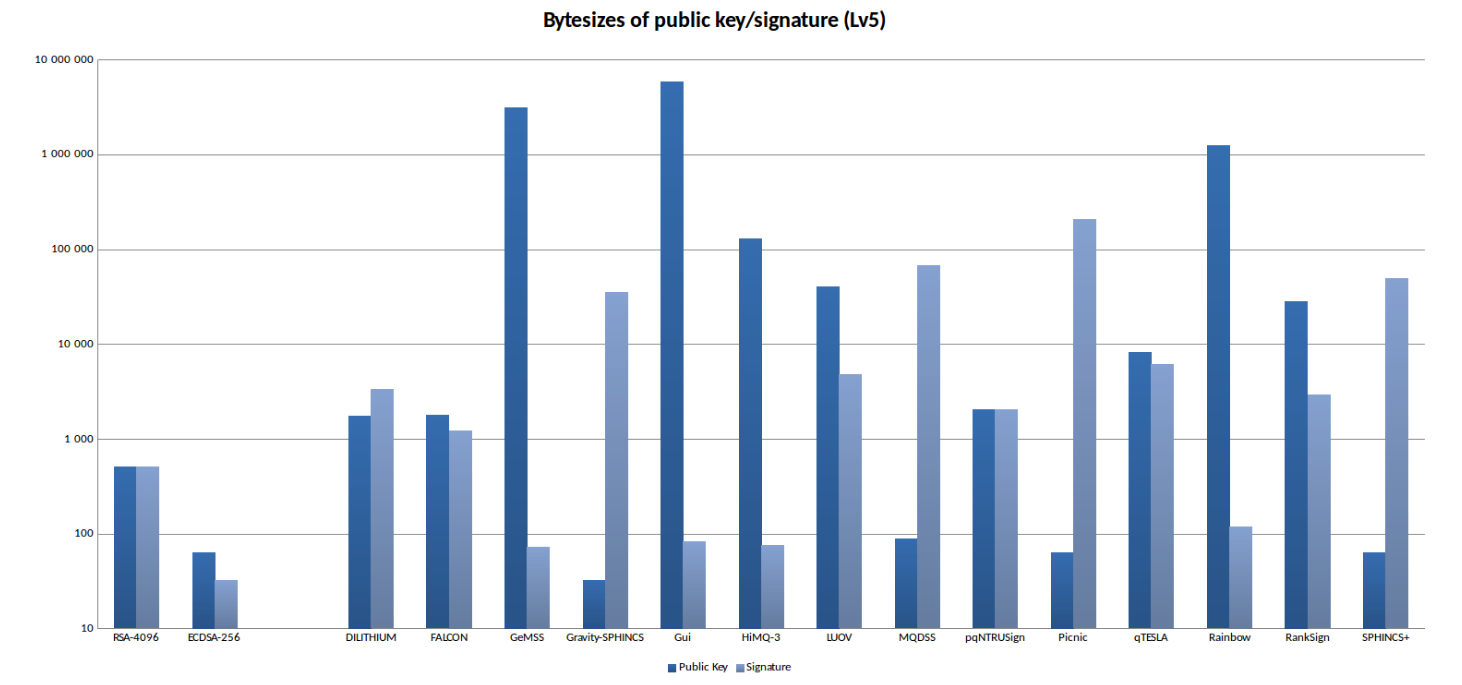
\includegraphics[width=80mm]{sizes.png}
		  \caption{Sizes of Post Quantum Signatures for 128 bit security}
		\label{fig:sizes}
		\end{center}
	 \end{figure}

	 Figure~\ref{fig:sizes} shows  public key and signature sizes for some post quantum cryptographies (cited from~\cite{falcon}).
	 You can see the total size never be under 1KB, most of them are even more thant 100 KBytes while ECDSA and RSA (non post quantum signatures) are around a few hundred of bytes.
	 Also for hash-based signature (e.g. XMSS or WOTS) we must consider about `state', which means we need to maintain how many times we sign with one public key.
	 This forces users to bother to care how many times their addresses were used.

    	
	\vspace{2.5mm}
	
	As such, we select lattice-based `BILSS' signature described in~\cite{bliss} and~\cite{blissb}. BLISS has relatively smaller public key and signature (around 1.7KB),
	and this is not stateful, so we can use one address as many times as we want.
	
	We stress again that using post quantum signature is a fight with its public key and signature size.
	We also note that unlike ECDSA and RSA, post quantum signatures are less flexible.
	Foe example we can use ECDSA and RSA  both as signature and key exchange and both are full homomorphic too, but practical post quantum cryptographies (e.g.\ BLISS) are not.
	So It does NOT MAKE SENSE AT ALL to compare with ECDSA-based cryptocurrencies (especially about sizes).

	\item\textbf{Strong Anonymity}\\ 
	In order to achieve anonymity, we utilize stealth address and coin mixing technique.
	These allow one to transact freely across iMesh, without the need to reveal one's address to either the receiver or to the wider network.
	\end{itemize}
	
	\section{BLISS Signature}
\label{sec:sig}
	
	As previously mentioned, Aidos Kuneen employs BLISS  as its signature algorithm.

BLISS is based on the hardness of Short Integer Solution (SIS) problem, 
and any efficient algorithms for solving SIS are  not known so the problem is hard even by quantum computers.

Formally SIS problem is defined as follows:

Let \( {\bf A} \in \mathbb{Z}^{n \times m}_{q} \) be an \( n \times m \) matrix with entries in \( \mathbb{Z}_{q} \) 
that consists of \( m \) uniformly random vectors  \( {\bf a_{i}} \in \mathbb{Z}^{n}_{q} : {\bf A} = |{\bf a_1}| \dots |{\bf a_m}| \).
Find a nonzero vector \( {\bf x} \in \mathbb{Z}^{m}\) such that: 
\begin{eqnarray}
	{\bf A}{\bf x}={\bf 0}  \in \mathbb{Z}^{n}_{q} \\
	|| {\bf x} || \le \beta 
\end{eqnarray}

In short find \( {\bf A}{\bf x}={\bf 0} \) for `small' \( {\bf x} \).

BLISS scheme can be described as a 3-rounds (commitment, challenge and response) identification protocol, known 
as  `\( \Sigma \)-protocol.' 
It is then transformed into a signature scheme by replacing the challenge generation step by a call to a hash function (modelled as a Random Oracle)
to generate the challenge.
	
\begin{figure}[ht]
	\begin{center}
	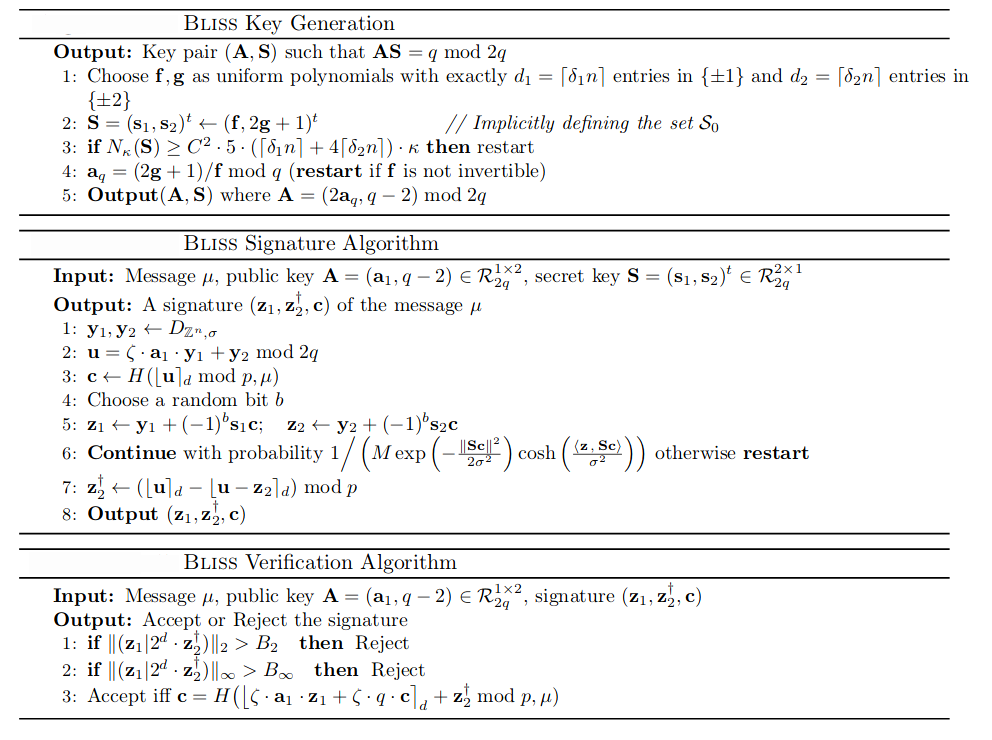
\includegraphics[width=80mm]{bliss.png}
	  \caption{BLISS Algorithm}
	\label{fig:bliss}
	\end{center}
 \end{figure}

 Figure~\ref{fig:bliss} shows the algorithm for BLISS signature. Intuitively,
 \begin{enumerate}
	\setlength\itemsep{0em}
\item Key Generation \\
Make a public key \( {\bf A} \) and a private key \( {\bf S} \) such that
\( {\bf A}{\bf S}=q \) mod \( 2q \)  with small \( {\bf S} \) 
\item Sign using \( \Sigma \) protocol
\begin{enumerate}
	\setlength\itemsep{0em}
	\item Pick random \( {\bf y_1} \) and \( {\bf y_2} \) from Gaussian distribution (variant: \( \sigma \))
\item Create a commitment  \( u = {\bf A}{\bf y_1} + {\bf y_2} \)
\item Create a challenge \( c \) by hasing \( u \) and message \( \mu \).
\item Create a response  \({\bf z_1} = {\bf y_1} + (-1)^{b}{\bf s_1}{\bf c}\) and  \({\bf z_2}= {\bf y_2} + (-1)^{b}{\bf s_2}{\bf c}\).
\item If \( {\bf z} \) is not in Gaussian distribution, restart from beginning of sign flow. This step is for preventing
leak of information about \( {\bf s} \). Intuitively this is because if \( {\bf z} \) follows Gaussian distribution, there is no way to
distinguish \( {\bf z} \)  from a random oracle from Gaussian distribution.
\item Output \( {\bf z} \) and \( {\bf c} \).
\end{enumerate}
\item Verification
\begin{enumerate}
	\setlength\itemsep{0em}
	\item Check \( {\bf z} \) is not too big.
	\item Calculate \( {\bf A}{\bf z} + q {\bf c} \) mod \(2q\) and get its hash.
	\item Check the above result is same as \( {\bf c} \).
	\end{enumerate}
 \end{enumerate}

The public key size \( {\bf A} \) is  870 bytes and is big for ADK address. We hash the public key and 
use the result as ADK address. Then the original public key is embedded into a signatures.

We note that after signing we use huffman coding to compress the signature. Since \( {\bf z}  \)  
distributes under Gaussian distribution with small deviation, we can assign less bits for smaller  \( {\bf z} \)
while assigning many bits for bigger values.
	
	\section{AKConsensus}
	\label{sec:AKConsensus}
	
	Each transactions in iMesh must be confirmed and the result of confirmation must be
	`Accepted' or `Rejected'. `Accepted' means that the transaction is valid and payment in the transaction takes place.
	`Rejected' means that the the transaction is one of double spend so is invalid. 

	We employ `AKConsensus' for confirming transactions. With AKConsensus, the confirmation processes
	are executed in parallel for fast confirmation by using DAG structure, since in DAG, we can efficiently maintain simultaneously
	confirmed transactions by leaves of iMesh,  unlike blockchain. This realizes zero lead-time confirmation unlike 
	other agreement based cryptocurrencies.

	AKConsensus utilizes  `multi valued byzantine agreement'
	described in~\cite{mba} for byzantine agreements by validators  whether transactions should be accepted or rejected.
	This agreement requires `binary byzantine agreement', which tries to agree with 
	'0' or '1'. We use~\cite{bba}  for this purpose. 
	We note that these agreement algorithm are tolerant to 1/3 adversaries (attackers).
	
	Figure~\ref{fig:bba} shows the algorithm of Binary Byzantine Agreement. The notations is as follows:

	\begin{figure}[ht]
		\begin{center}
		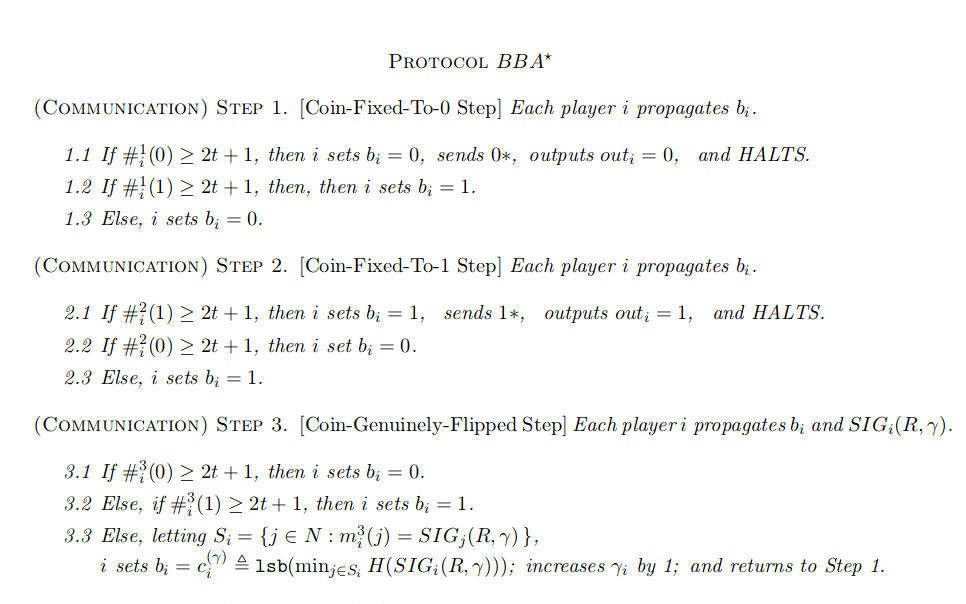
\includegraphics[width=80mm]{bba.png}
		  \caption{Binary Byzantine Algorithm}
		\label{fig:bba}
		\end{center}
	 \end{figure}

	 \begin{itemize}
		\setlength\itemsep{0em}
		\item  The set of all players (validators) is \(N\),  the cardinality of \(N\) is \(n\),  the number of malicious players is \(t\),
		 and \( n= 3t+ 1\).
		 \item We identify each player \( i \) with his public key.  We denote \(i\) ’s digital signature of a string \(x\) by \(sig_{i}(x) \).
		  To ensure signers and messages are retrievable from digital signatures, we define \\
				\( SIG_{i} (x) = (i,x,sig_i(x) )\)
		  \item For all rounds \(r\) and players \(i\) and \(j\), in a BA protocol \(i\) receives a single message from \(j\), denoted by \(m^r_i(j)\),
  				either an element of \(V \) or the symbol \( \bot \notin V \).
  		  \item For each possible value \(v\) we denote by \( \#^{r}_{i}(v) \) the number of players from which \(i\) has received the value \(v\).
	 \end{itemize}

	 We use BLISS signature explained in Section~\ref{sec:sig} for \(sig_{i}(x) \). 
	
	 \vspace{2.5mm}

	 The algorithm for Multi Valued Byzantine Agreement is as follows. Note that 
	 a process is said to be perplexed if, in the first round, it receives at least as many as \( (n - t) /2 \) initial values different from its own.
	 Processes that are not perplexed are said to be content. 
	 \begin{enumerate}
		\setlength\itemsep{0em}
		 \item Each validator sends its initial value  to every other process. 
		 \item Each `perplexed' process sends a message to every other process. The semantics of this message is just `I am perplexed'.
		 \item Each validators set `alert' flag true if and only if at least as many as \(n-2t\) players  are claiming they are perplexed.
		 \item The binary agreement is used to reach agreement on `alert' flag.
\begin{itemize}
	\setlength\itemsep{0em}
	\item If the binary agreement agrees alert = true, all correct processes use a predefined default value as the result.
		 \item If agreement is alert = false, then the value of content processes  is the result of the agreement.
		 Perplexed processes deduce this result by using the initial value that is common to a majority of the content processes. 
\end{itemize}
	 \end{enumerate}
	
In AKconsensus values that validators can select are `Pend', `Reject' and `Accept', and the default value is `Pend'.

	\vspace{2.5mm}
	
	Finally the whole process of AKConsensus is as follows:
	
	\vspace{-0.5\baselineskip}
	\begin{enumerate}
		\setlength\itemsep{0em}
		\item Each nodes defines the addresses of trusted nodes within their trusted list.
		\item A new transaction arrives to a validator, the validator determine the value \(v \)  it should propose (i.e. `Pend', `Reject' or `Accept') 
		by checking the status of inputs of the transaction:
		\begin{enumerate}
			\setlength\itemsep{0em}
			\item If one of the inputs is already consumed, the transaction is conflicting and another conflicting transaction was already accepted.
			\(v \)  will be `Reject'.
			\item If one of the inputs is  locked, then another conflicting transactions are now trying agreement. \(v \) will be `Pend'
			\item Otherwise \(v \)  is `Accept'
		\end{enumerate}	
		\item The validator locks all inputs of the transaction to remind that the transaction which consume these inputs is now under agreement.
		\item The validator proposes  the value \(v\) (`Pend', `Reject' and `Accept') and tries to agree on one value  by Multi Valued Byzantine Agreement.
		\item After agreement finishes the validator frees all locks of inputs. 
		\item If the result of agreement is `Accepted' or `Rejected', the validator marks it in its database.
	\end{enumerate}
	
	This agreements are done in parallel by utilizing the feature of DAG structure, where we can confirm many transactions simultaneously.
New transactions  only refers already `Accepted' transactions as its parent so we can maintain all accepted transactions by leaves of iMesh, and we don't need to 
send all (hashes of) accepted transactions when we need to inform accepted transactions to others.


We note that if some transactions are once agreed on `Pend' (due to existence of conflicting transactions), we retry to agree on these transactions in lexicographical order of these hashes.
If \(2/3\) validators follows the rule the transaction whose hash is lexicographically smallest in conflicting transactions will be successfully confirmed and others will be rejected.

	\vspace{1.5mm}
	
	
	\section{Proof of Work}
	\label{sec:PoW}
	
	When sending a transaction, senders must first perform `Proof of Work' (PoW), similar to that which is performed by miners in the 
	Bitcoin network. The mandatory performance of PoW prior to sending a transaction is necessary in order to protect iMesh from DDoS 
	attacks via spam transactions. During the PoW operation each transaction is assigned a length \(L\), of 32-bit integer fields known as a `nonce'. 
	The value of this nonce is set such that the hash of the block will contain a leading run of zeros and form a series of `Cuckoo Graphs' with cycle length \(L\) (as is discussed in more detail below). The leading run of zeroes determines the time required for the PoW operation and has been chosen to produce an 
	average PoW time of a few minutes.
	
	\vspace{2.5mm}
	
	For PoW operations, Aidos Kuneen implements the Cuckoo Cycle as discussed in~\cite{cuckoo}. The Cuckoo Cycle arises by the insertion of
	keys into a `Cuckoo Hashtable' which naturally leads to the cyclic formation of random bipartite graphs. A Cuckoo Hashtable consists of 
	two identical tables, each with a unique hash function which maps a key to a table location (this provides two possible locations for 
	each key). Upon arrival of a new key, its table location is first determined. If both possible locations are currently occupied by 
	existing keys, then one is extracted and inserted into its alternate location (potentially displacing yet another key). This process is 
	subsequently repeated until either a vacant location is identified, or a predetermined number of iterations is reached. This process 
	leads to the formation of cycles in what is referred to as a `Cuckoo Graph'. The Cuckoo Graph is a bipartite graph with a node at each 
	location, and an edge for every inserted key, connecting the two locations at which the key can reside.

	\begin{figure}[ht]
		\begin{center}
		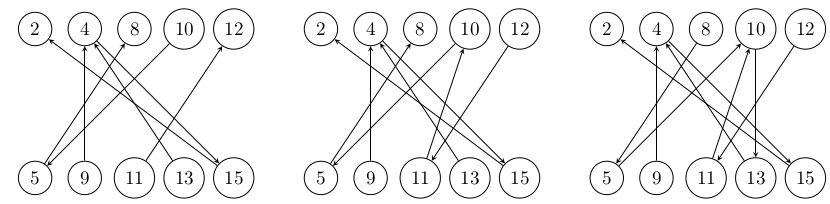
\includegraphics[width=80mm]{cuckoo.png}
		  \caption{Cuckoo Graph}
		\label{fig:cuckoo}
		\end{center}
	 \end{figure}
	
	\vspace{-3.5mm}
	
	The first diagram in Figure~\ref{fig:cuckoo} illustrates the directed Cuckoo Graph on \( N = 8 + 8 \) nodes after edges (2, 15), (4, 
	9), (8, 5), (4, 15), (12, 11), (10, 5) and (4, 13) are added. In order to add the 8th edge (10, 11), we follow the paths \( 10 
	\rightarrow 5 \rightarrow 8 \) and \( 11 \rightarrow 12 \) to find the different roots 8 and 12. Since the latter path is shorter, we 
	reverse the path to \( 12 \rightarrow 11\) such that we can add the new edge as (\( 11 \rightarrow 10\)), resulting in the middle 
	diagram. In order to add the 9th edge (10, 13) we now find the path from 10 to be the shorter one, so we reverse the path and add the 
	new edge as (\( 10 \rightarrow 13\)), resulting in the right diagram. When adding the 10th edge (8, 9), we find the paths
	 \( 8 \rightarrow 5 \rightarrow 10 \rightarrow 13 \rightarrow 4  \rightarrow 15 \rightarrow 2 \) and \( 9 \rightarrow 4 \rightarrow 15 
	 \rightarrow 2 \)  with equal roots. In this case, we can compute the length of the resulting cycle as 1 plus the sum of the path lengths to the node where the two paths join. In the diagram, the paths join at node 4, and the cycle length is computed as 1 + 4 + 1 
	 = 6.
	
	\vspace{2.5mm}
	
	The Cuckoo Cycle has been chosen as the PoW function for iMesh, due to the following reasons:
	
	\begin{itemize}
		\setlength\itemsep{0em}
	\item We anticipate significantly higher daily transaction volumes compared to that of Bitcoin, this is due to the fact that unlike Bitcoin, the fee-less nature of Aidos Kuneen means the economic disincentive against frequently sending small transactions is removed. Thus, Aidos Kuneen requires a very fast verification method.
	\item Unlike other typical PoW algorithms such as Cryptonight or Scrypt which are typically quite resource intensive, full-nodes are able to verify the validity of nonces much faster when utilizing the Cuckoo Cycle. 
	\item Unlike Bitcoin, in which PoW is performed only on the blocks themselves, in Aidos Kuneen PoW must be performed for each individual transaction. As there are significantly more individual transactions than there are blocks, Aidos Kuneen therefore requires more power to perform PoW verification. Thus, it is essential that a highly efficient means of verification, such as the Cuckoo Cycle is employed.
	\item In order to prevent an attacker from being able to propagate fraudulent transactions throughout the network, specialist hardware such as ASICs and FPGAs should not provide any advantage. As the PoW time is mainly dominated by memory access speed, specialist processing hardware is essentially rendered ineffective.
	\item Cuckoo Cycle is the most memory bound so is immune from quantum speedup by Grover's search algorithm.
	\end{itemize}
	
	The following Cuckoo Cycle parameters will be used for PoW operations:
	
	\begin{itemize}
		\setlength\itemsep{0em}
		\item cycle length \( L\) = 20 (To minimize the size impact on transactions).
		\item number of nodes \( N = 2^{25} \) (To provide memory usage of around 128MB\@).
		\item easiness \(N/M = 100\% , (M\): number of edges) (To prevent optimizations by edge trimming).
	\end{itemize}
	
	\section{Ticket Mining}
	\label{sec:mining}
	

	\begin{figure}[ht]
		\begin{center}
		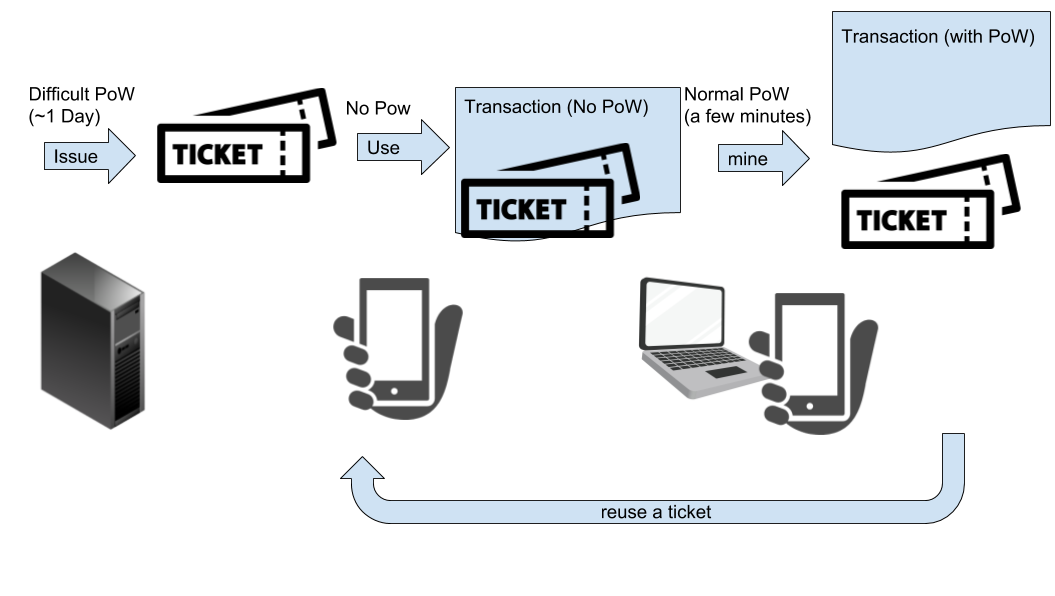
\includegraphics[width=80mm]{ticket.png}
		  \caption{Ticket Flow}
		\label{fig:ticket}
		\end{center}
	 \end{figure}
	

	To cater specifically for IoT devices (whose performance is typically quite low), we introduce a `ticket mining' mechanism for co-operative Proof of Work without fee.

Figure~\ref{fig:ticket} shows a flow of using tickets.

	`Ticket issuers' try to issue tickets out of thin air by difficult PoW than one for normal transactions. Once issued the issuer sends a transaction with the ticket without PoW.
	The transaction will never be taken into iMesh without PoW.
	Other `miners' try to mine the transaction with normal difficulty PoW for getting the ticket, once mined the transaction will be taken into iMesh and the miner gets the ticket.
	The miner can reuse the ticket for sending his/her transaction without PoW.

	By utilizing tickets, senders can do PoW in free time for mining tickets and once  tickets are mined they can send transactions immediately without PoW.

	Normally tickets are mined by PC or servers with high performance. Once these tickets are used, these will be mined by IoT devices or normal PC, and the tickets are used with
	IoT devices or phones. Since it just takes a few minutes to do normal PoW, even IoT devices have good chances to mine transactions successfully.

	Optionally we utilize fee-based transaction for people who don't want to issue and mine tickets. In fee-based transaction we use fee instead of a ticket, and miners
	try to mine the transaction for getting the fee.
	
	\section{AKShuffle}
	\label{sec:aks}
	
	For increased anonymity we employ \emph{AKShuffle}. Within AKShuffle we utilize stealth address for unlinkable transactions
	and coin mixing for untraceable payments.


	\subsection{Stealth Address}

	We use stealth address technique inspired by~\cite{ringsig}. The stealth address
	explained in~\cite{ringsig} uses full homomorphism of ECDSA and  Elliptic Curve Diffie Hellman (ECDH) key exchange,
	but unfortunately	BLISS signature is NOT homomorphic\footnote{Since another post quantum signature, 
	Ring-LWE signature is somewhat homomorphic, we could use it for stealth address. But this
	would make signature size much bigger than BLISS (1.7KB \(\rightarrow\) 4KB)}.
	We modify the technique to not use
	homomorphism and replace ECDH  to post quantum cryptography `Supersingular Isogeny Key Exchange' (SIKE).

	A sender and receiver exchange a secret key that a sender made with SIKE and the sender sends ADK to the public key which is made from the secret key.
	No one except the sender and receiver cannot get to know the secret key.
	Then the receiver can receive the ADK since he knows the secret key. We show the detailed flow as follows:

	\begin{enumerate}
		\setlength\itemsep{0em}
		\item A receiver show his SIKE public key.
		\item A sender makes a random secret key.
		\item The sender makes a key pair (private key and public key) of BLISS from his secret key above.
		\item The sender makes a transaction which sends ADK to the BLISS public key above.
		\item The sender encrypts his secret key with receiver's SIKE public key and embeds it into the transaction as `exchange key'.
		\item The receiver checks exchange keys in transactions and picks up ones which are encrypted by his SIKE public key.
		\item The receiver decrypts the secret key from the exchange key.
		\item The receiver makes a key pair (private key and public key) of BLISS from the secret key above.
		\item The receiver makes his own new BLISS public / private key pair.
		\item The receiver sends ADK in the transaction above to his own public key.
	\end{enumerate}

	Note that unlike stealth addresses with ECDSA, a private key made by a sender is shared with the sender and the receiver.
	Thus the receiver must send ADK again to his own public key to not be used later by the sender  maliciously.

	\subsection{Coin mixing}

	Recent ECDSA-based cryptocurrencies like Monero or MimbleWimble use confidential transactions with mixing techniques (e.g.\ ring signature or mixing commitments themselves).
	But unfortunately the confidential transaction includes range proof~\cite{bullet}, which utilizes commitment scheme with full homomorphism.
	To the best of our knowledge there are not practical post quantum commitment schemes with full homomorphism.
	
Once we choose to not use confidential transaction, it is not well practical only to mix sender addresses.
This is because all input amounts in a transaction must be all same for anonymizing all senders.
We could form ring signature scheme with BLISS and Ring-LWE signature by replacing their ZKNI (Zero Knowledge Non interactive) signature proof, but we don't use
it due to the above reason and its size (estimated around 20KB--40KB).

	Instead we use fee incentive coin mixing  technique for  untraceable payments instead.
	We stress that we  sacrifice less for anonymity since coin mixing is a off-chain solution.	
	On the other hand, some anonymous cryptocurrencies sacrifices something, for example, their transaction size or convenience (e.g.\ they remove public address and
	senders must always ask receiver's address when sending). 

	\vspace{2.5mm}

We apply DiceMix technique described in~\cite{mixing} for mixing outputs. By DiceMix we mix outputs of a transaction 
without letting others (including owners f the transaction outputs) know who is holding which outputs  .


DCnet is the core of DiceMix which make players publish  their  own  message anonymously. 
We assume that messages to be mixed are encoded as elements of a finite field \( \mathbb{F} \) with \( |\mathbb{F}|> n \), 
where \( n\) is the number of peers \( P \). Given \( n\) slots, each peer \(i\),  with  message \(m_i\), 
publishes \(m_j^i\) (i.e. \(m_i\) to  the \(j\)-th power)  in  the \(j\)-th  slot. 
This  yields  an  intentional  collision involving  all  peers  in  each  of  the  slots.
 Using  addition in  \( \mathbb{F} \) to  create  DCnet  messages,  the \(j\) -th  slot contains the power sum \( S_j=\Sigma_{i}m_j^i\).

 Now, we require a mechanism to extract the messages \( m_j\) from  the  power  sums \(S_j\).
 Let \( g(x) = a_{n}x^{n}+a_{n-1}x^{n-1}+ \cdots a_1x+a_0 \) 
 be  a  polynomial  with  roots \(m_1,m_2 \cdots m_n\). Newton’s identities  state 
 \begin{eqnarray*}
	a_n&=& 1 \\
	a_{n-1}&=&-S_1 \\
	a_{n-2}&=& (a_{n-1}S_1-S_2)/2 \\
	a_{n-3}&=& -(a_{n-2}S_{1}-a_{n-1}S_2+S_3)/3 \\
	\cdots&
 \end{eqnarray*}
	By knowledge of all coefficients \( a_j\) of the polynomial \(g\), we can find its \(n\) roots, which are the \(n\) input messages

	\vspace{2.5mm}

	The detailed flow of mixing is as follows.

\begin{enumerate}
	\setlength\itemsep{0em}
	\item Participants, who want to send ADK anonymously, or want to get fee, join AKShuffle network and waits for senders, who want to send ADK
	with fee.
	\item A sender broadcasts an offer about 
	\begin{itemize}
		\setlength\itemsep{0em}
		\item Session ID
		\item Amount he wants to send anonymously
		\item Fee he will pay for each participants
		\item An UTXO (Unspent Transaction Output) he will use (The UTXO also plays as an user ID).
		\item Signature signed with UTXO address for ensuring that the he is the owner of the UTXO
		\item Number of transaction inputs he wants.
		\item Output address for change
		\item SIKE public key
	\end{itemize}
	\item Participants checks the offer and if a participant can pay the amount and is happy about the fee, reply with a message including:
	\begin{itemize}
		\setlength\itemsep{0em}
		\item An UTXO he will use (The UTXO also plays as an user ID).
		\item Output address for change
		\item SIKE public key
	\end{itemize}
	\item The sender checks the messages  and after he  collects enough participants, he sends information about:
	\begin{itemize}
		\setlength\itemsep{0em}
		\item UTXOs of participants the sender selected (as user ID)
		\item Encrypted oracle secret key with participants' SIKE public key. 
		This data is included only for participants with lexicographically less UTXO bytes than one of the sender.
	\end{itemize}
	\item Each participants check the messages above  and they reply with encrypted oracle secret as described above.
	Now each participants and the sender exchanged secrets with each other by SIKE.
	\item They start to exchange their outputs by DCnet protocol. \\
	We assume a player with user ID \(my\) wants to include her output \(m_{my} \) and has exchanged secret \(k(p)\) with player with user ID \(p\). 
	She calculates DCSLOTPAD = \( \Sigma_{p \in P} sgn (my-p) * k(p) \in \mathbb{F} \),
	where \(sgn(my-p)\) is 1 if lexicographically \(my > p\), otherwise -1. And she calculates. 
		 \(  DC_{my,s} = {m_{my}}^s + DCSLOTPAD \) for each slots \( s = 1 \cdots n+1 \).
	 \item Each players sends hash of \( DC_{my,s}\) for committing before sending \(DC_{my,s}\).
	 \item Each players sends  \( DC_{my,s}\).
	 \item Each players calculate \( M_s = \Sigma_{i} DC_{i,s} \) for each slots \(s\). Notice that the term  DCSLOTPAD  will be canceled
	and  \(M_s = \Sigma_{i} m_{i}^s \).
	\item Calculate \(m_{i}\) by DCnet explained before.
	\item Each players sorts outputs \(m_{i}\) and make a transaction including the outputs.
	\item Each players checks received transactions are all same.
	\item Each players does PoW and sends the result.
	\item Each players sends the transaction into iMesh.
\end{enumerate}

We are expecting the fee will be lower and even be zero, once ADK will be matured and there will be
many participants who are willing to mix inputs without fee.

	\section{Network}
	\label{sec:network}
	
	\begin{figure}[ht]
		\begin{center}
		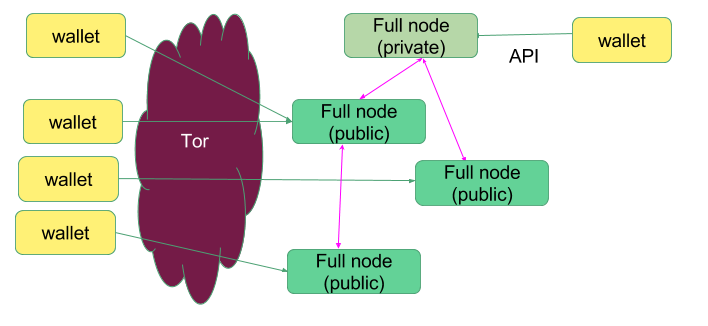
\includegraphics[width=80mm]{network.png}
		  \caption{Aidos Kuneen network topology}
		\label{fig:network}
		\end{center}
	 \end{figure}
	
	\vspace{-3.5mm}
	
	
	As illustrated in Figure~\ref{fig:network}, the Aidos Kuneen network is comprised of a series of full-nodes who communicate in a P2P fashion. 
	Clients can either connect directly to these full-nodes or to their own full-node via API\@. Clients are able to send API requests in order to broadcast their transactions to the network (this is usually performed automatically
	by the wallet application). Between full-nodes, transactions are sent and received using protocol buffer\footnote{https://developers.google.com/protocol-buffers/}, 
	which is one of most efficient serializer in order to reduce packet sizes.
	
	\vspace{2.5mm}
	
	In order to ensure anonymity between public full-nodes and clients we utilise the Tor network. This is essential as full-nodes
	may otherwise receive sensitive information such as their clients' IP addresses along with the clients' transactions.  
	
	\vspace{2.5mm}
	
	It is important to note that Tor is not employed for communications between full-nodes. This is due to the fact that routing traffic via the Tor network introduces an unavoidable element of delay into inter-nodal communications, and efficiency between full-nodes 
	is a critical aspect of the speed of the entire Aidos Kuneen network. Additionally, there is little need to enforce anonymous communication between nodes, this is due to the fact that even if the initial client-to-node connection were not secured with Tor, the initial receiving node 
	does not transmit any sensitive information about the client when it relays the transaction to the other nodes.
	
	\vspace{2.5mm}
	
	Unfortunately however, Tor is not quantum secure. Though, Tor does have the advantage of being a well established, trusted network with a large number of participants. We believe that for the short term at least, the strong anonymity provided 
	by the Tor network is an excellent fit for Aidos Kuneen. We will continue to investigate other potential methods of providing quantum-resistant anonymity as they become available. 
	
	\vspace{2.5mm}
	
	Table~\ref{tbl:cmd} lists the basic packet commands for the Aidos Kuneen network.
	
	 \begin{table}[htb]
		\caption{Basic Packet Commands}
		\label{tbl:cmd}
		\begin{tabularx}{\linewidth}{XX} 
			command & description \\
			\toprule
			version & inform version and that we are preparing connection \\
			verack & acknowledge of version \\
	  ping & ping to another node \\
	  pong & response of ping \\
	  get\_addr & get node addresses\\
	  addr & response node addresses \\
	  inv &  invent new transaction hashes \\
	  get\_data & request transaction contents \\
	  txs & respond transaction contents \\
	  get\_leaves & request  leaves' hashes \\
	  leaves &  respond leaves' hashes \\
	  get\_following\_hash &  request transaction hashes around a specified transaction in iMesh\\
	  following\_hash &  respond of get\_following \_hash \\
	  consensus\_message & message for consensus, sent by validators \\
	  \bottomrule
	\end{tabularx}
	  \end{table}

	  \section{Conclusion}
	  We summarize features of Aidos Kuneen in Table~\ref{tbl:spec}.
  	
	\begin{table}[htb]
		\caption{Aidos Kuneen: Technical Specifications}
		\label{tbl:spec}
		\begin{tabularx}{\linewidth}{XX} 
			\toprule
			Ticker & ADK \\
			\midrule
	Total Supply & 25,000,000 ADK \\ 
	\midrule
	Minimum Unit & 0.00000001 (\(10^{-8})\) ADK \\ 
	\midrule
	PoW Algorithm & Cuckoo Cycle\\ 
	\midrule
	Anonymity & AKShuffle and Tor \\
	\midrule
	Consensus Algorithm & AKConsensus \\ \midrule
	Distributed Ledger & iMesh (transaction DAG) \\
	\midrule
	Signature Scheme & BLISS (post quantum lattice based signature)\\ 
	\midrule
	Usage &  Finance, Banking, Digital Commerce, IoT Micropayments \\ 
	\bottomrule
	\end{tabularx}
	  \end{table}
	
	% \vspace{3cm}
	
	% \begin{center}
	% 
\includegraphics[width=40mm]{logo-min}
	% \end{center}
	
	 
	\twocolumn[
		\begin{@twocolumnfalse}
	
	
	  \begin{thebibliography}{99}
		
		\bibitem{btc}
			Satoshi Nakamoto,
			\emph{Bitcoin: A Peer-to-Peer Electronic Cash System}, 2008.
		
		\bibitem{iota}
		Serguei Popov,
			\emph{The tangle}, 2017.
		
		\bibitem{prob}
		Sheldon M. Ross,
			\emph{Introduction to Probability Models. 10th Edition}, 2012.
		
				
		\bibitem{shor}
		Peter W. Shor, 
			\emph{Polynomial-Time Algorithms for Prime Factorization and Discrete Logarithms on a Quantum Computer}, 1995.
			
		\bibitem{google}
		Masoud Mohseni, Peter Read, Hartmut Neven,
			\emph{Commercialize early quantum technologies}, 2017.
			
		\bibitem{recom}
		PQCRYPTO,
			\emph{Post-Quantum Cryptography for Long-Term Security, Initial recommendations of long-term secure post-quantum
			systems}, 2015.
				
		\bibitem{ringsig}
		Nicolas van Saberhagen,
			\emph{CryptoNote v 2.0}, 2013.
	
		\bibitem{cuckoo}
		John Tromp,
			\emph{Cuckoo Cycle: a memory bound graph-theoretic proof-of-work}, 2014.
	
		\bibitem{pqcrypto}
			PQCRYPTO,
				\emph{Post-Quantum Cryptography for Long-Term Security}, 2015.	
		
		\bibitem{bliss}
			L\'{e}o Ducas and Alain Durmus and Tancr\`{e}de Lepoint and Vadim Lyubashevsky,
				\emph{Lattice Signatures and Bimodal Gaussians}, 2013.
		
		\bibitem{blissb}
		L\'{e}o Ducas 
				\emph{Accelerating Bliss\@: the geometry of ternary polynomials}, 2014.		

		\bibitem{falcon}
		Pierre-Alain Fouque, Jeffrey Hoffstein, Paul Kirchner, VadimLyubashevsky, Thomas Pornin,Thomas Prest, Thomas Ricosset,Gregor Seiler, William Whyte and Zhenfei Zhang,
				\emph{Falcon}, (\url{https://tprest.github.io/Slides/falcon-polsys.pdf}).

		\bibitem{bba}
		Silvio Micali,
				\emph{Byzantine Agreement, Made Trivial}, 2018
			
		\bibitem{mba}
		R.Turpin and  B.Coan,
				\emph{Extending binary Byzantine agreement to multivalued Byzantineagreement}, 1984
		
		\bibitem{sis}
		Wikipedia,
				\emph{Short integer solution problem}, (\url{https://en.wikipedia.org/wiki/Short_integer_solution_problem})
		
		\bibitem{bullet}
		Benedikt B\"{u}nz, Jonathan Bootle, Dan Boneh,Andrew Poelstra, Pieter Wuille, and Greg Maxwell,
				\emph{Bulletproofs: Short Proofs for Confidential Transactions and More}, 2017
		
		\bibitem{mixing}
		Tim Ruffing, Pedro Moreno-Sanchez, Aniket Kate
				\emph{P2P Mixing and Unlinkable Bitcoin Transactions}, 2016

					\end{thebibliography}
		\end{@twocolumnfalse}
]
	

	\end{document}
	
